\documentclass[11pt,a4paper]{article}

\usepackage[margin=2.5cm]{geometry}
\usepackage[T1]{fontenc}
\usepackage[utf8]{inputenc}
\usepackage{lmodern}
\usepackage{amsmath,amssymb}
\usepackage{graphicx}
\usepackage{booktabs}
\usepackage{caption}
\usepackage{tikz}
\usetikzlibrary{positioning,arrows.meta}
\usepackage[hidelinks]{hyperref}

\graphicspath{{figures/}}
\captionsetup{font=small,labelfont=bf}

\title{Baseline: On-Device Forecasting and Language Models\\
for Personal Health Ranges on iOS}
\author{Nikola Jankovikj (259076)\\[2pt]\small Smart Mobile Applications}
\date{November 2026}

\begin{document}
\maketitle

\begin{abstract}
Smartwatches record resting heart rate, heart-rate variability, breathing rate and wrist temperature every night, but the phone apps that show these numbers rarely say whether a value is unusual \emph{for this person}, or what to do about it. We present \emph{Baseline}, an iOS app that learns each user's expected range for every metric and notices when the readings leave it. Everything runs on the device.

A pretrained time-series foundation model, Chronos-2-small, is exported to Core ML (28\,MB, int8) and forecasts an expected range for each day from the user's Apple Health history. Deterministic Swift rules turn deviations into a readiness score and flagged events such as an illness warning or sustained strain. The on-device Apple Intelligence language model explains the flags, suggests what to do about an out-of-range value, writes a weekly report and answers free-text questions. Every model output passes through an output guard, and a template takes its place whenever the guard rejects it.

The Core ML model matches the PyTorch reference to within 2.6\% of the forecast band, and one 32-series call takes about 55\,ms on an M3 CPU. On synthetic data the foundation model is as accurate as a 28-day moving average, which agrees with our earlier thesis result. Its value in the app is practical: ranges from the first days, missing values handled, and multi-step horizons. The main engineering lesson concerns the language model. It is useful only when code does all comparisons and numbers and the model just puts them into words, and that design has to be re-checked after every OS update.
\end{abstract}

% ---------------------------------------------------------------------------
\section{Introduction}

Consumer wearables have made overnight physiology a commodity. An Apple Watch writes resting heart rate, heart-rate variability (HRV), respiratory rate, wrist temperature and sleep duration to Apple Health every morning. Changes in these signals often come before symptoms of illness~\cite{mishra2020covid,radin2020influenza}, and HRV responds to training load and stress~\cite{shaffer2017hrv}. Most apps, however, show the raw values against population norms or against a plain average. Users then have to judge for themselves whether 63\,bpm is high for \emph{them}, and what to do about it.

This project builds a mobile app that does that judgement on the phone. In an earlier project~\cite{jankovikj2026chronos} we tested whether the zero-shot forecasts of Chronos-2~\cite{ansari2025chronos2} can serve as a personal reference for anomaly detection on wearable data. They can, but no better than a simple average. Baseline takes the method to a phone, with two further aims:

\begin{enumerate}
  \item \textbf{Personal ranges on the device.} Forecast an expected range per metric and day from the user's own history, with no server, account or network access, and show it next to a simple-average range so the user can see what the model adds.
  \item \textbf{Actionable explanations.} When a value falls outside its range, say in plain language what happened and what to do, using the on-device language model~\cite{apple2025afm,apple_foundationmodels} without letting it invent numbers or diagnose.
\end{enumerate}

\paragraph{Contributions.} We export Chronos-2-small to a single fixed-shape Core ML program and check that it matches PyTorch to within a stated tolerance (Section~\ref{sec:forecast}). We design a pipeline from forecast to flag whose expected ranges stay frozen during multi-night deviations (Section~\ref{sec:rules}). We build a language-model layer in which code decides and the model only words the result, protected by an output guard and backed by templates (Section~\ref{sec:llm}). Finally, we test the whole app automatically on macOS and in the iOS simulator, including against the live language model (Section~\ref{sec:eval}).

% ---------------------------------------------------------------------------
\section{Background and related work}

\paragraph{Wearables for early detection.} Mishra et al.~\cite{mishra2020covid} showed that resting heart rate measured by smartwatches rises before symptoms in most COVID-19 cases. Radin et al.~\cite{radin2020influenza} found that population resting heart rate tracks influenza-like illness. Both detect deviations from a \emph{personal} baseline, usually a rolling median with a fixed threshold, and both run on a server.

\paragraph{Forecasting-based anomaly detection.} A forecaster predicts the next values of a series, and large standardised residuals are anomalies~\cite{hundman2018telemanom}. Chronos~\cite{ansari2024chronos} and Chronos-2~\cite{ansari2025chronos2} are pretrained time-series foundation models that forecast new series zero-shot and output quantiles. Chronos-2 also accepts covariates and processes groups of related series jointly. Our thesis~\cite{jankovikj2026chronos} found that its residuals separate lab stress from rest with a median AUROC of about 0.96. A context mean did just as well, and covariates did not help.

\paragraph{On-device language models.} Since iOS 26 the Foundation Models framework exposes Apple's on-device model of about 3B parameters~\cite{apple2025afm}. It offers \emph{guided generation}, where a Swift type marked \texttt{@Generable} constrains decoding to that type's schema, and \emph{tool calling}. The model is small, has a 4{,}096-token context, and is updated with the operating system, which matters later.

% ---------------------------------------------------------------------------
\section{Architecture}

The app is a SwiftUI app for iOS 26 and later. Everything that is not a screen lives in a local Swift package, \texttt{BaselineKit}, with four modules (Table~\ref{tab:modules}). The package's tests run on the Mac in about half a minute without a simulator, which kept the development loop short. Figure~\ref{fig:arch} shows the data flow.

\begin{figure}[t]
  \centering
  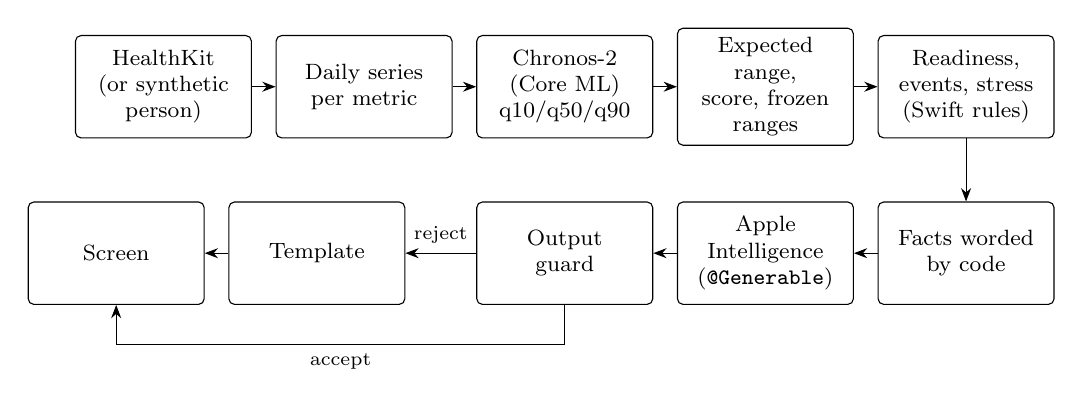
\begin{tikzpicture}[node distance=3mm, >=Stealth,
      box/.style={draw, rounded corners=2pt, align=center, text width=20mm,
                  minimum height=13mm, font=\footnotesize}]
    \node[box] (a) {HealthKit\\ (or synthetic\\ person)};
    \node[box, right=of a] (b) {Daily series\\ per metric};
    \node[box, right=of b] (c) {Chronos-2\\ (Core ML)\\ q10/q50/q90};
    \node[box, right=of c] (d) {Expected range,\\ score, frozen\\ ranges};
    \node[box, right=of d] (e) {Readiness,\\ events, stress\\ (Swift rules)};
    \node[box, below=8mm of e] (f) {Facts worded\\ by code};
    \node[box, left=of f] (g) {Apple\\ Intelligence\\ (\texttt{@Generable})};
    \node[box, left=of g] (h) {Output\\ guard};
    \node[box, left=9mm of h] (i) {Template};
    \node[box, left=of i] (j) {Screen};
    \foreach \src/\dst in {a/b, b/c, c/d, d/e, e/f, f/g, g/h} \draw[->] (\src) -- (\dst);
    \draw[->] (h) -- (i) node[midway, above, font=\scriptsize]{reject};
    \draw[->] (i) -- (j);
    \draw[->] (h.south) |- ++(0,-5mm) -| node[pos=0.25, below, font=\scriptsize]{accept} (j.south);
  \end{tikzpicture}
  \caption{Data flow. The top row produces every number and flag; the bottom row only puts them into words.}
  \label{fig:arch}
\end{figure}

\begin{table}[t]
  \centering\small
  \caption{Code organisation.}
  \label{tab:modules}
  \begin{tabular}{lp{11.5cm}}
    \toprule
    Module & Responsibility \\
    \midrule
    \texttt{HealthData} & Metric definitions, the \texttt{HealthDataProvider} protocol, the HealthKit provider, and a seeded synthetic person with scripted scenarios \\
    \texttt{Forecasting} & Core ML wrapper and batching, simple average, frozen ranges, readiness, event rules, stress estimate, backtest \\
    \texttt{Insights} & Facts for the language model, templates, guided generation, the output guard, metric advice, the Ask chat \\
    \texttt{Persistence} & Journal (manual logs, feedback, stored explanations) and forecast cache as two JSON files, CSV export \\
    \texttt{App} & App state (\texttt{AppModel}), the screens, background refresh, notifications \\
    \bottomrule
  \end{tabular}
\end{table}

One \texttt{@Observable} \texttt{AppModel} owns the state. A refresh reads up to 400 days of history, forecasts and scores the most recent 38 days so that the Today screen can appear, then fills in the rest of the six months in the background. Explanations are generated last. A refresh that is already running is cancelled and replaced, so changing a setting (data source, demo scenario, forecast mode) takes effect at once and no result from the previous source reaches the screen.

We stored data as two JSON documents rather than in SwiftData. The app never queries its own data. It reads and writes the journal and the forecast cache whole, and a schema and model context would add code for no benefit.

% ---------------------------------------------------------------------------
\section{Implementation}

\subsection{Health data}
\texttt{HealthKitProvider}~\cite{apple_healthkit} reads eight daily metrics: resting heart rate, HRV, respiratory rate, wrist temperature, sleep duration, steps, active energy and VO$_2$max. It also reads workouts and the last 36 hours of heart rate and steps for the stress estimate. It writes the user's alcohol logs back to Health. Because the simulator's Health store is empty, a \texttt{SyntheticProvider} generates a person whose overnight signals share a slow ``strain'' state that reacts to the previous day's training load. Scripted events sit at fixed distances from today. There are three scenarios: a \emph{sick week} that ends in four nights of illness-like signals, a \emph{healthy} history, and a \emph{first days} history with only nine nights. A SplitMix64 generator makes the data identical on every platform, so tests and screenshots are repeatable.

\subsection{Chronos-2 on iOS with Core ML}\label{sec:forecast}
Chronos-2 is published as a PyTorch model with a Python pipeline around it. iOS runs neither, so the forecaster had to become a Core ML model that the app calls from Swift. This section describes how, since the same steps apply to other PyTorch time-series models.

\paragraph{The model.} \texttt{chronos-2-small} is an encoder-only transformer with about 28M parameters: 6 layers, model width 512, 8 attention heads. A series is normalised by its own mean and standard deviation, squashed with $\operatorname{arcsinh}$, and cut into patches of 16 steps. Each patch becomes one token, together with a time encoding and a mask of which steps were observed. A learned \texttt{[REG]} token and one token for the future patch follow. Every layer attends twice: \emph{along time}, within one series with rotary position embeddings, and \emph{across the group}, between series at the same time step. The second attention lets one call forecast related series jointly and use covariates. The future token is decoded into 13 quantile levels (q01 to q99) for the next 16 steps.

\paragraph{Why it cannot be converted as it is.} Core ML compiles a static graph from a traced model, and the stock forward pass resists tracing in four ways. Missing values are NaN, and the model removes them with \texttt{nanmean}, which Core ML lacks. Shapes depend on the input: the context length, the number of patches and the size of each group change from call to call. Padding, group ids and the time encoding are computed in Python outside the model. And the graph uses operations without a Core ML equivalent, such as \texttt{asinh}, as well as attention masks filled with the smallest float32, which turns into $-\infty$ under reduced precision.

\begin{table}[t]
  \centering\small
  \caption{Core ML export against PyTorch. Error is $|\text{Core ML}-\text{PyTorch}|$ as a fraction of the q10--q90 width; latency is the median 32-row call on an M3 CPU.}
  \label{tab:parity}
  \begin{tabular}{lccccc}
    \toprule
    & & & \multicolumn{2}{c}{Error, q10--q90} & Max error, \\
    \cmidrule(lr){4-5}
    Weights & Size (MB) & Latency (ms) & max & mean & all 13 levels \\
    \midrule
    float32 & 112.1 & 54 & 0.000 & 0.000 & 0.000 \\
    \textbf{int8 (shipped)} & \textbf{28.4} & \textbf{55} & \textbf{0.026} & \textbf{0.004} & \textbf{0.117} \\
    palette6 & 21.2 & 58 & 0.058 & 0.007 & 0.198 \\
    palette4 & 14.2 & 54 & 0.260 & 0.040 & 0.600 \\
    \bottomrule
  \end{tabular}
\end{table}

\paragraph{A fixed-shape restatement.} We therefore wrote \texttt{Chronos2Export}, a PyTorch module of about 180 lines that reuses the original weights and computes the same function with only fixed shapes and plain operations:

\begin{itemize}
  \item \textbf{Fixed shapes.} One call takes 32 rows of 512 context steps and returns 32 rows of 13 quantiles over 16 steps. The inputs are \texttt{context} (32$\times$2$\times$512), \texttt{known\_future} (32$\times$2$\times$16) and \texttt{group\_ids} (32). Channel 0 of each input holds the values and channel 1 holds 1 where a value was observed.
  \item \textbf{Masks instead of NaN.} Mean and standard deviation are sums weighted by the observed channel, and a patch with no observed value is masked out of attention. A shorter history is left-padded as unobserved. This is exact rather than an approximation: unobserved patches are never attended to, rotary embeddings depend only on relative position, and the time encoding counts back from the start of the forecast. An unused row is all unobserved and sits alone in its own group.
  \item \textbf{Precomputed tables.} With the shape fixed, the rotary $\cos$/$\sin$ tables, the time encodings and the \texttt{[REG]} embedding are constants stored in the model rather than computed in it. No shape is read back from a tensor, because the converter cannot fold the integer casts that tracing such reads produces.
  \item \textbf{Plain operations.} $\operatorname{arcsinh}(x)$ is written as $\operatorname{sign}(x)\log(|x|+\sqrt{x^2+1})$, which avoids the cancellation that $x+\sqrt{x^2+1}$ suffers for negative $x$. Masked attention scores get $-10^4$, which gives the same softmax and stays finite at any precision. Group attention carries no position, since the rows of a group have no order.
\end{itemize}

\paragraph{Conversion.} The module is traced with \texttt{torch.jit.trace} and converted by coremltools~\cite{coremltools} into an ML Program for iOS 18 and later. The model computes in float32. In float16, instance normalisation squares raw values, and the square of a day's step count overflows. The 13 quantile levels are stored in the model's metadata, so the app finds q10, q50 and q90 by level rather than by position. The export script, about 230 lines, also generates golden fixtures. These are six forecasting tasks run through the stock PyTorch pipeline: a nine-day cold start, a history longer than the context, a series with a quarter of its values missing, a constant series, two targets forecast jointly, and a target with past and known-future covariates.

\paragraph{Compression.} Table~\ref{tab:parity} compares weight compressions against the PyTorch pipeline on these fixtures. Each variant is saved, loaded from disk on the CPU as the app runs it, and measured. The app reads q10, q50 and q90, so our tolerance is a maximum error below 5\% of the q10--q90 width at those levels. We ship int8 weights with per-channel symmetric quantisation: a quarter of the size, within tolerance, and no slower. Six-bit palettisation would save another 7\,MB but just misses the tolerance (0.058). Four-bit palettisation is off by up to a quarter of the band. Compression costs most at q01 and q99, which the app does not use. The script refuses to install a shipped variant that fails the tolerance, and a Swift test asserts the same tolerance against the same fixtures on every test run.


\paragraph{Running it in the app.} \texttt{Chronos2Forecaster} is a Swift actor around the model, about 200 lines.
\begin{itemize}
  \item \textbf{Loading.} The package ships the \texttt{.mlpackage} as exported. \texttt{swift build} has no Core ML compiler, so the app compiles the model on first use with \texttt{MLModel.compileModel} and keeps the result in Caches. The cached copy is named after the package's model identifier, so a new export is compiled again. The input shapes are read from the model description, so a re-export with another row count or context length needs no code change.
  \item \textbf{Compute units.} The model runs on the CPU only. The Neural Engine does not run float32, and a background task may not use the GPU.
  \item \textbf{Batching.} A forecasting task is one or more target series with optional covariates. Tasks are packed into 32-row calls, one group id per task. In the default per-metric mode each metric and forecast day is a one-row task, so one call covers four days of all eight metrics. In joint mode a day's metrics, the user's logs and a weekend flag share one group id.
  \item \textbf{Reading the output.} q10, q50 and q90 become the expected range. Neighbouring quantiles of a compressed model can cross by a hair, so the three are sorted before use.
\end{itemize}
Section~\ref{sec:eval} reports the cost of a call. The app logs its own forecasting time on every refresh.

\subsection{Expected ranges and scores}
For each metric and day, the \emph{expected range} is the forecast's q10--q90 and the \emph{score} is the standardised residual from the thesis,
\begin{equation}
  z = \frac{y - q_{0.5}}{\hat\sigma}, \qquad \hat\sigma = \frac{q_{0.9}-q_{0.1}}{2.563}.
\end{equation}

\paragraph{Frozen ranges.} A rolling forecaster adapts to a deviating night and then calls the next one normal. A four-night illness would then show as a single flagged night. While values stay clearly outside the range ($|z|\geq2$), Baseline therefore keeps the range forecast \emph{before} the run began and reads it further ahead each night, for up to seven nights. After that the deviation is taken as the new normal. This is the thesis's fixed personal reference, which was what made sustained stress detectable there, and it is why the model's multi-step horizon matters. Forecasts are cached by series and date, so after the first launch a refresh only forecasts the new day.

\paragraph{The simple-average comparison.} Every chart can overlay the range a 28-day mean and standard deviation would give. A \emph{Model check} screen backtests both forecasters, and per-metric versus joint forecasting, on the user's own history and reports error and coverage.

\subsection{From forecast to flag}\label{sec:rules}
Fixed rules turn the scores into what the user sees. Nothing is flagged until 14 nights of data exist; until then the ranges are shown as provisional.
\begin{itemize}
  \item \textbf{Readiness (0--100)} is a weighted mean of per-signal logistic scores in each signal's \emph{concern} (its score towards the side that can signal strain). The weights are 0.3 for HRV and resting heart rate, 0.2 for sleep, and 0.1 each for respiratory rate and temperature. A signal exactly as expected scores 88, one at $2\sigma$ on the concerning side 34.
  \item \textbf{Events.} An \emph{illness warning} is at least two of resting heart rate, respiratory rate and temperature above range on two or more consecutive nights. \emph{Sustained strain} is heart rate up and HRV down for three nights. A \emph{deviation} is any other stretch that includes a clear deviation. A single mild night for one metric happens every few weeks by chance and is not an event.
  \item \textbf{``Consider talking to a clinician''} is set by a rule (four nights of illness warning, or any signal at $5\sigma$) and shown from that flag. The language model is told never to say it.
  \item \textbf{Stress estimate.} Daytime heart rate in 5-minute bins is forecast from the recent resting heart rate and steps. Bins with sleep, workouts or movement are excluded, and episodes above the forecast are reported as an estimate.
\end{itemize}

\subsection{The language-model layer}\label{sec:llm}
The model is used in four places: the explanation of a flagged event, the advice for an out-of-range value, the weekly report, and the Ask chat. They follow one principle, \emph{code decides and the model words}, which we arrived at by running the model and watching it fail:

\begin{itemize}
  \item \textbf{Comparisons are worded by code.} Given bare numbers, the model misjudged which side of a range a value was on. It now receives sentences such as ``64\,bpm, above the expected 55--59'', with signals above and below their range in separate lists. Given one mixed list, it called everything ``elevated''.
  \item \textbf{Relative days are worded by code.} Left to work out dates, the model called a night two days back ``last night''. Facts say ``yesterday (Thu 12 Nov)'' where that is true, and the model may only repeat it.
  \item \textbf{Facts stay facts.} In the weekly report the model writes only the headline and the focus for the coming week. The lists of what went well and what was flagged come from code; when it was allowed to choose, the model praised metrics that had got worse.
  \item \textbf{Guided generation.} Outputs are \texttt{@Generable} structs, for example \texttt{AnomalyInsight} with a summary, one to three likely contributors and one suggestion. Greedy sampling makes the same facts always give the same text.
\end{itemize}

\paragraph{Output guard.} \texttt{InsightGuard} accepts a text only if (i) every number in it occurs in the facts, compared by value so that ``7'' matches ``7,0''; (ii) it contains no diagnosis or medication terms from a list of stems; (iii) no sentence places a signal on the opposite side of its range from the facts; and (iv) ``last night'' and ``yesterday'' appear only where the facts use them. A rejected text is replaced by a template written from the same facts. The templates are also what the app shows without Apple Intelligence, so every screen works without it.

\paragraph{Advice where the value is.} The first version explained only flagged events, and the user had to open the Insights tab to learn anything. So that a value outside its range comes with a suggestion where the user sees it, the metric detail screen now shows a \emph{What to do} card whenever the day in focus is outside its range (Figure~\ref{fig:advice}, left). Code decides whether the reading is the better or worse side for that metric: higher HRV is better, higher resting heart rate is worse, and fewer steps is worse. It collects context from the user's logs and workouts, such as alcohol logged the evening before or a 95-minute run. The template advice for that metric and side appears at once. The model's version, which links the reading to the context, replaces it when it is ready and accepted. Scrubbing across the chart waits 400\,ms before starting a generation, and results are cached until the next refresh.

\paragraph{Ask: three agents.} Ask is a chat about the user's own data. Each message passes through three model sessions, each with its own short instructions:

\begin{enumerate}
  \item \textbf{Triage.} A guided-generation call sorts the message into a greeting, a question about the user's data, or something else. For greetings and off-topic messages the model writes a short reply itself. For an off-topic message it says that the app is not a general assistant and does not attempt the question. A message made only of small-talk words (``thanks'', ``ok great'') skips triage. After an answer, the model had sorted ``thanks'' as a follow-up question, and the app answered the previous question again.
  \item \textbf{Research.} A second session gets five tools: one night's sleep, a metric over recent days, workouts, logs, and what was flagged. Each tool returns a summary worded by code, as described above, and its text reply is discarded. Only the calls count. Each call appears in the chat as it is made (``Sleep: Last night (Sun, 15 Nov to Mon, 16 Nov)''), so the user sees what is being looked up while waiting. Tool choice is still the model's weak point (Section~\ref{sec:eval}). To cover for it, the summaries that the question's keywords point to are always added, and a follow-up such as ``what should I do about it?'' inherits the previous question's keywords.
  \item \textbf{Writer.} A third session streams the answer from the lookups alone. It gives the direct answer first and then a few plain sentences on what it means. Expected ranges and numbers are left out unless the user asks for detail. A suggestion must address something that is outside its range; if nothing is, the user is told to carry on as usual. The guard checks the finished text. If it fails, the model retries once and is told what was wrong (``used numbers that are not in their data (6.5)''). If that also fails, the app shows the lookups themselves.
\end{enumerate}

\noindent Under the answer, a disclosure lists every lookup with its result. Without Apple Intelligence, keyword routing answers directly with the matching summaries.

\begin{figure}[t]
  \centering
  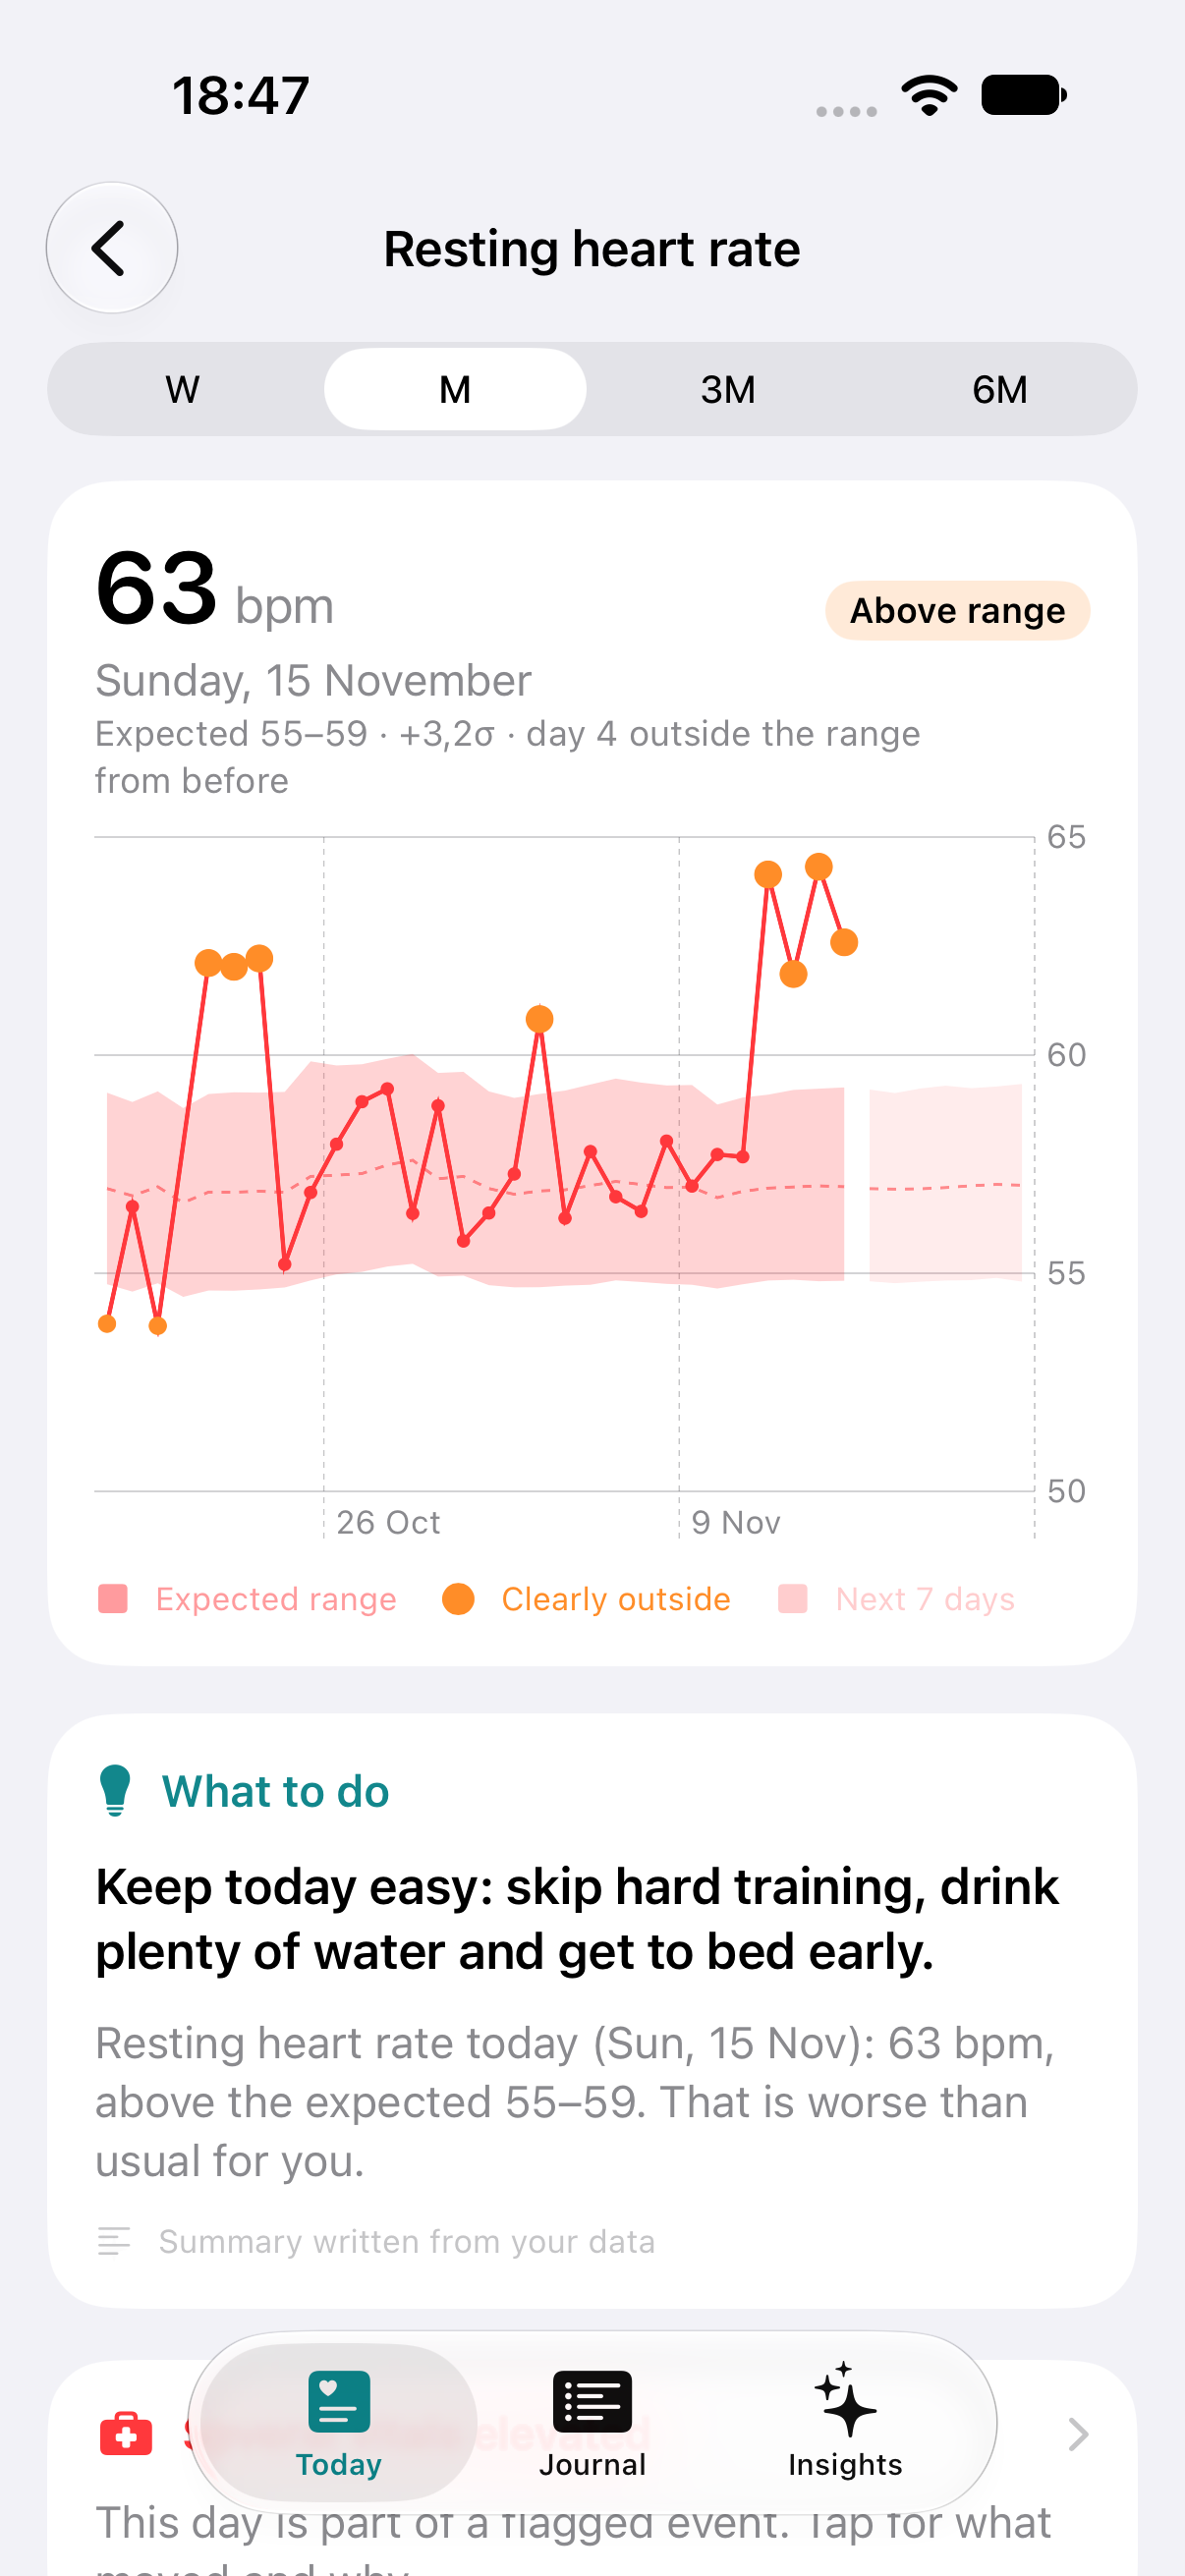
\includegraphics[width=0.3\textwidth]{metric-advice.png}\hspace{1.5em}
  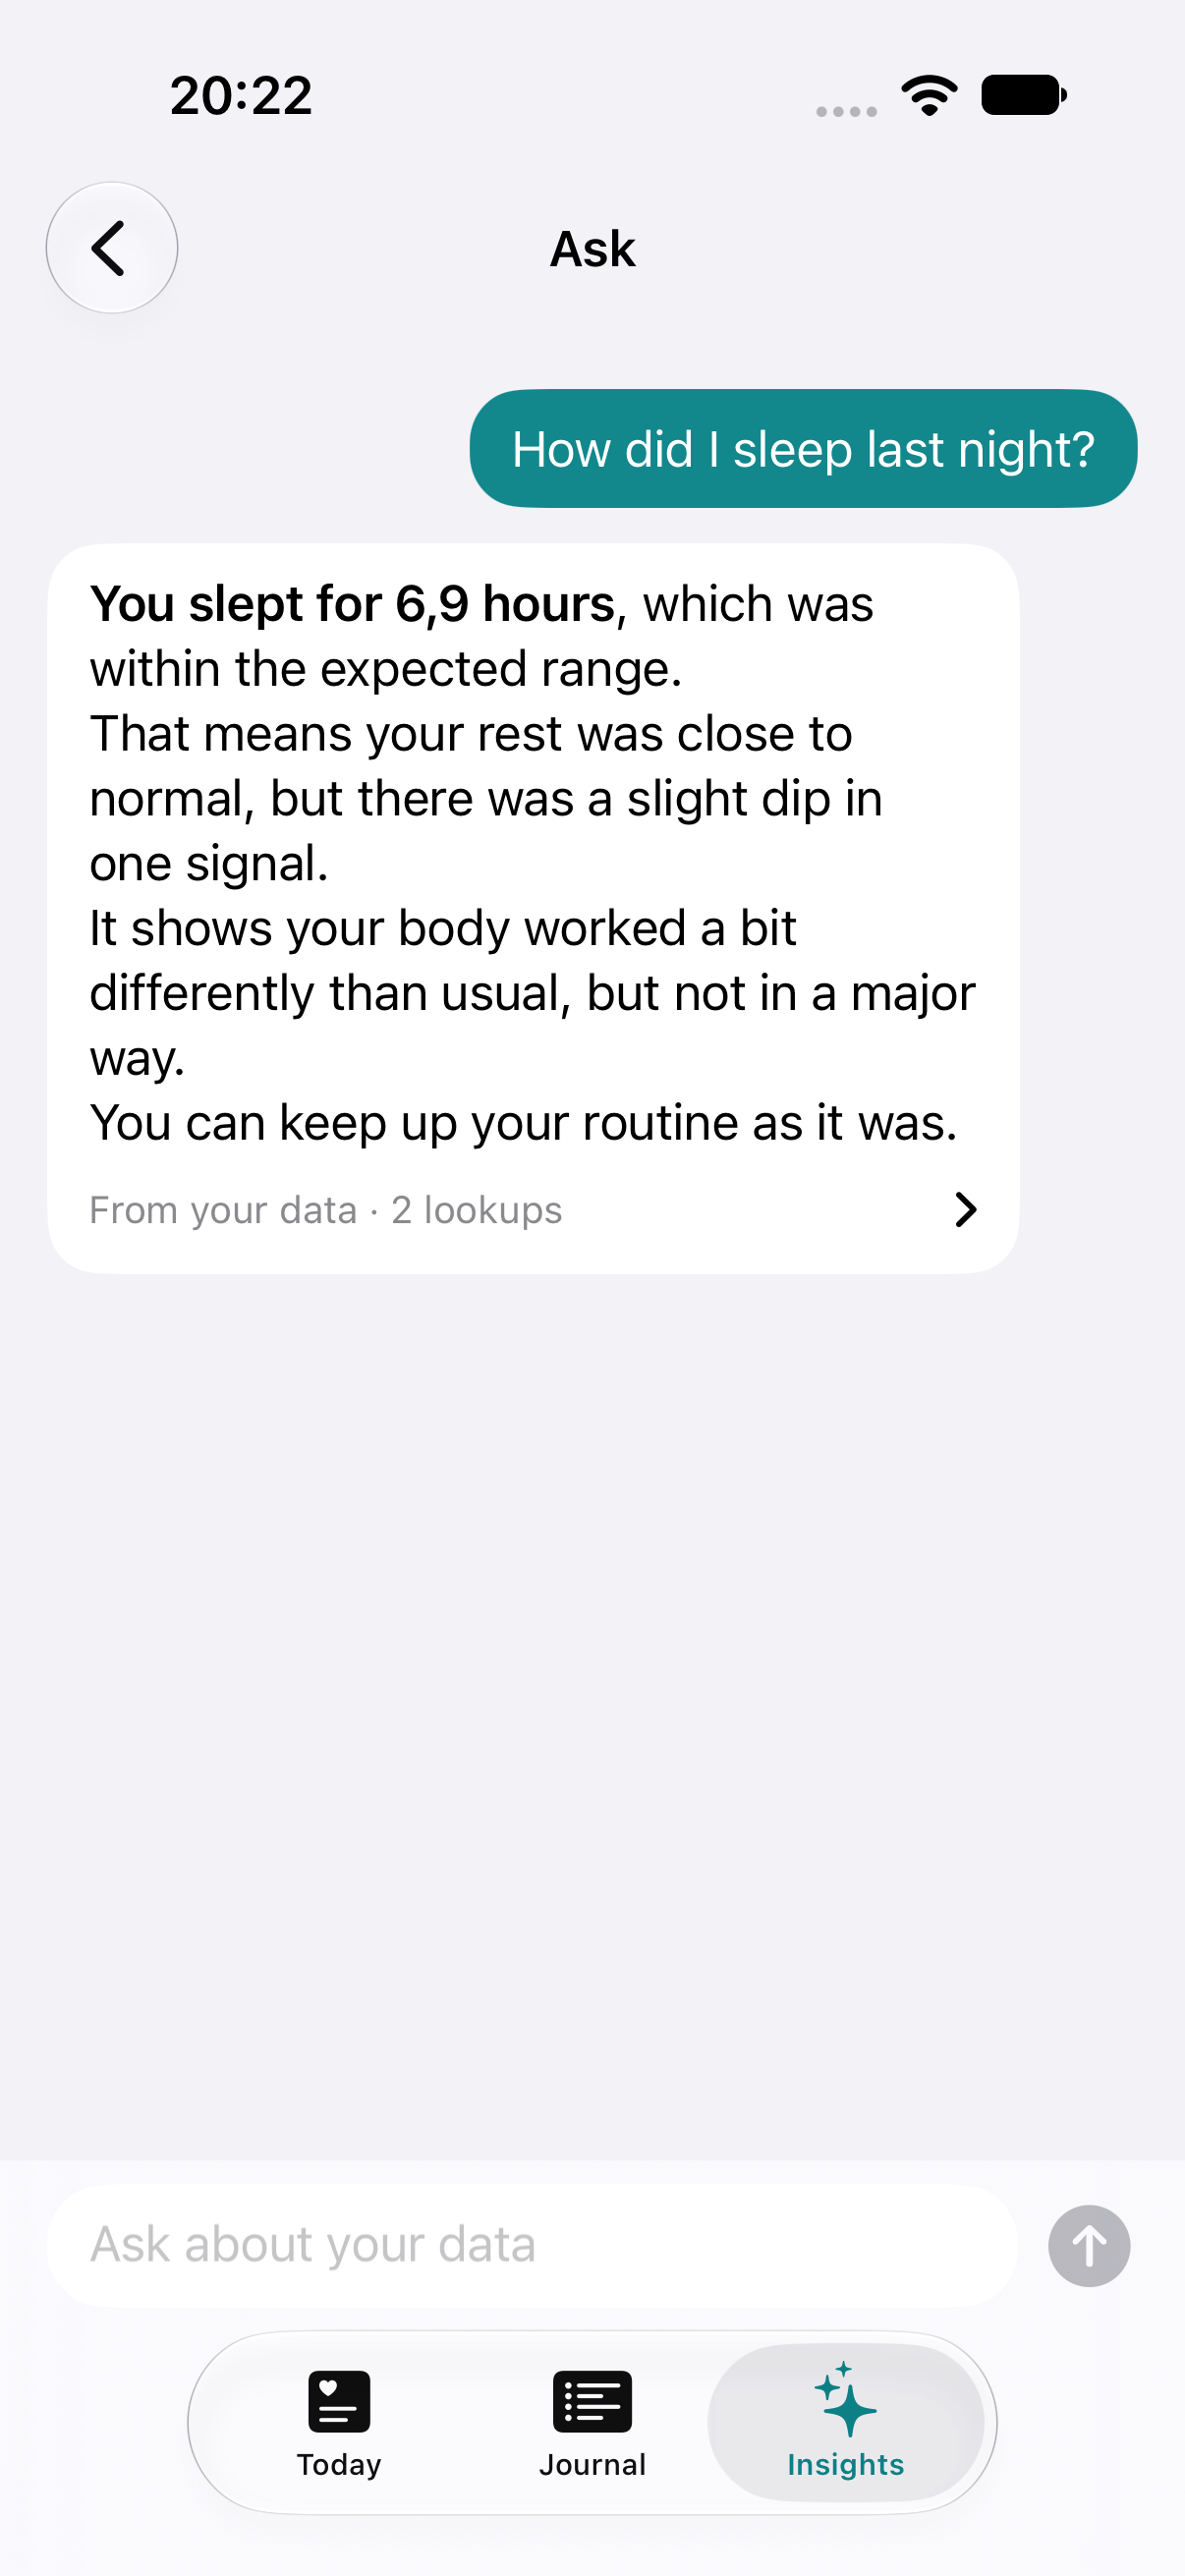
\includegraphics[width=0.3\textwidth]{ask.png}
  \caption{Left: an out-of-range resting heart rate with its advice card on the metric screen. Right: an Ask answer streamed by the writer agent, with the research agent's lookups one tap away (``From your data $\cdot$ 2 lookups'').}
  \label{fig:advice}
\end{figure}

\subsection{User interface}
The app has three tabs (Figure~\ref{fig:screens}). \textbf{Today} shows readiness with its contributing signals, the current event with its explanation, the stress estimate, and a tile with a two-week sparkline per metric. Tapping a tile opens the \textbf{metric detail}, a Swift Charts plot over a week, month, three or six months, with the shaded expected range, the next seven days' outlook, an optional simple-average overlay, and the advice card. \textbf{Journal} lists flagged events and one-tap manual logs (alcohol, caffeine, feeling sick, stress, hard training, travel). Each event screen shows what moved and the explanation, and asks ``Does this make sense?'' so the user can tag a cause. Their tags become context for the next explanation. \textbf{Insights} holds the weekly report and Ask. Each generated text says whether Apple Intelligence or a template wrote it.

\begin{figure}[t]
  \centering
  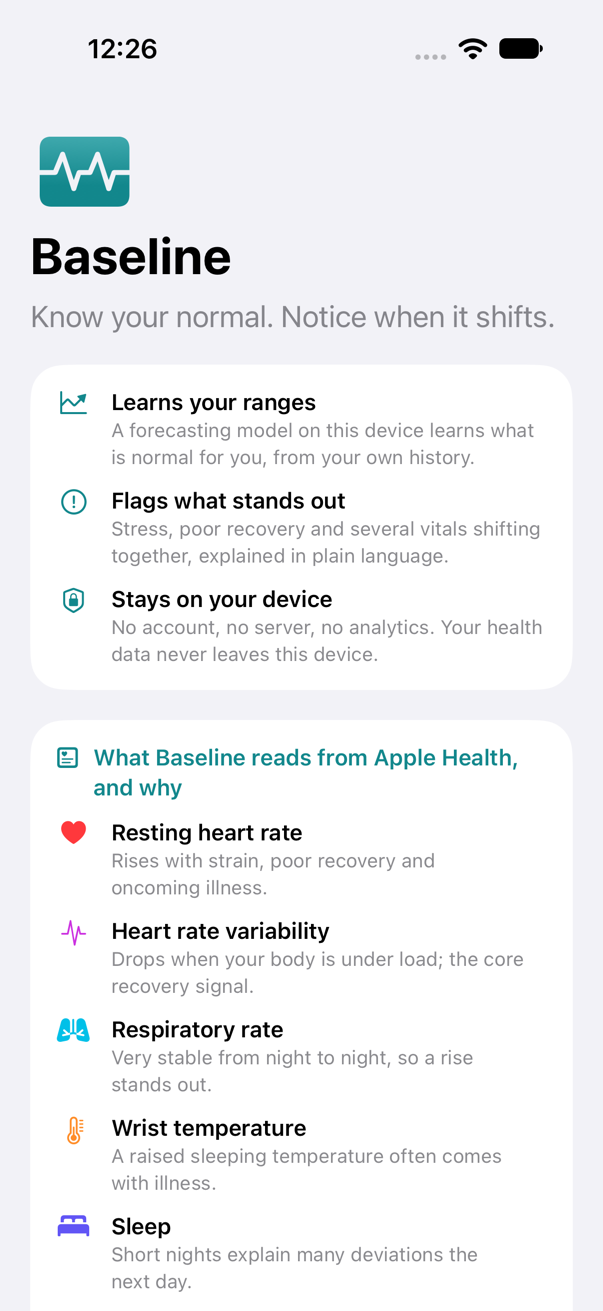
\includegraphics[width=0.19\textwidth]{onboarding.png}\hfill
  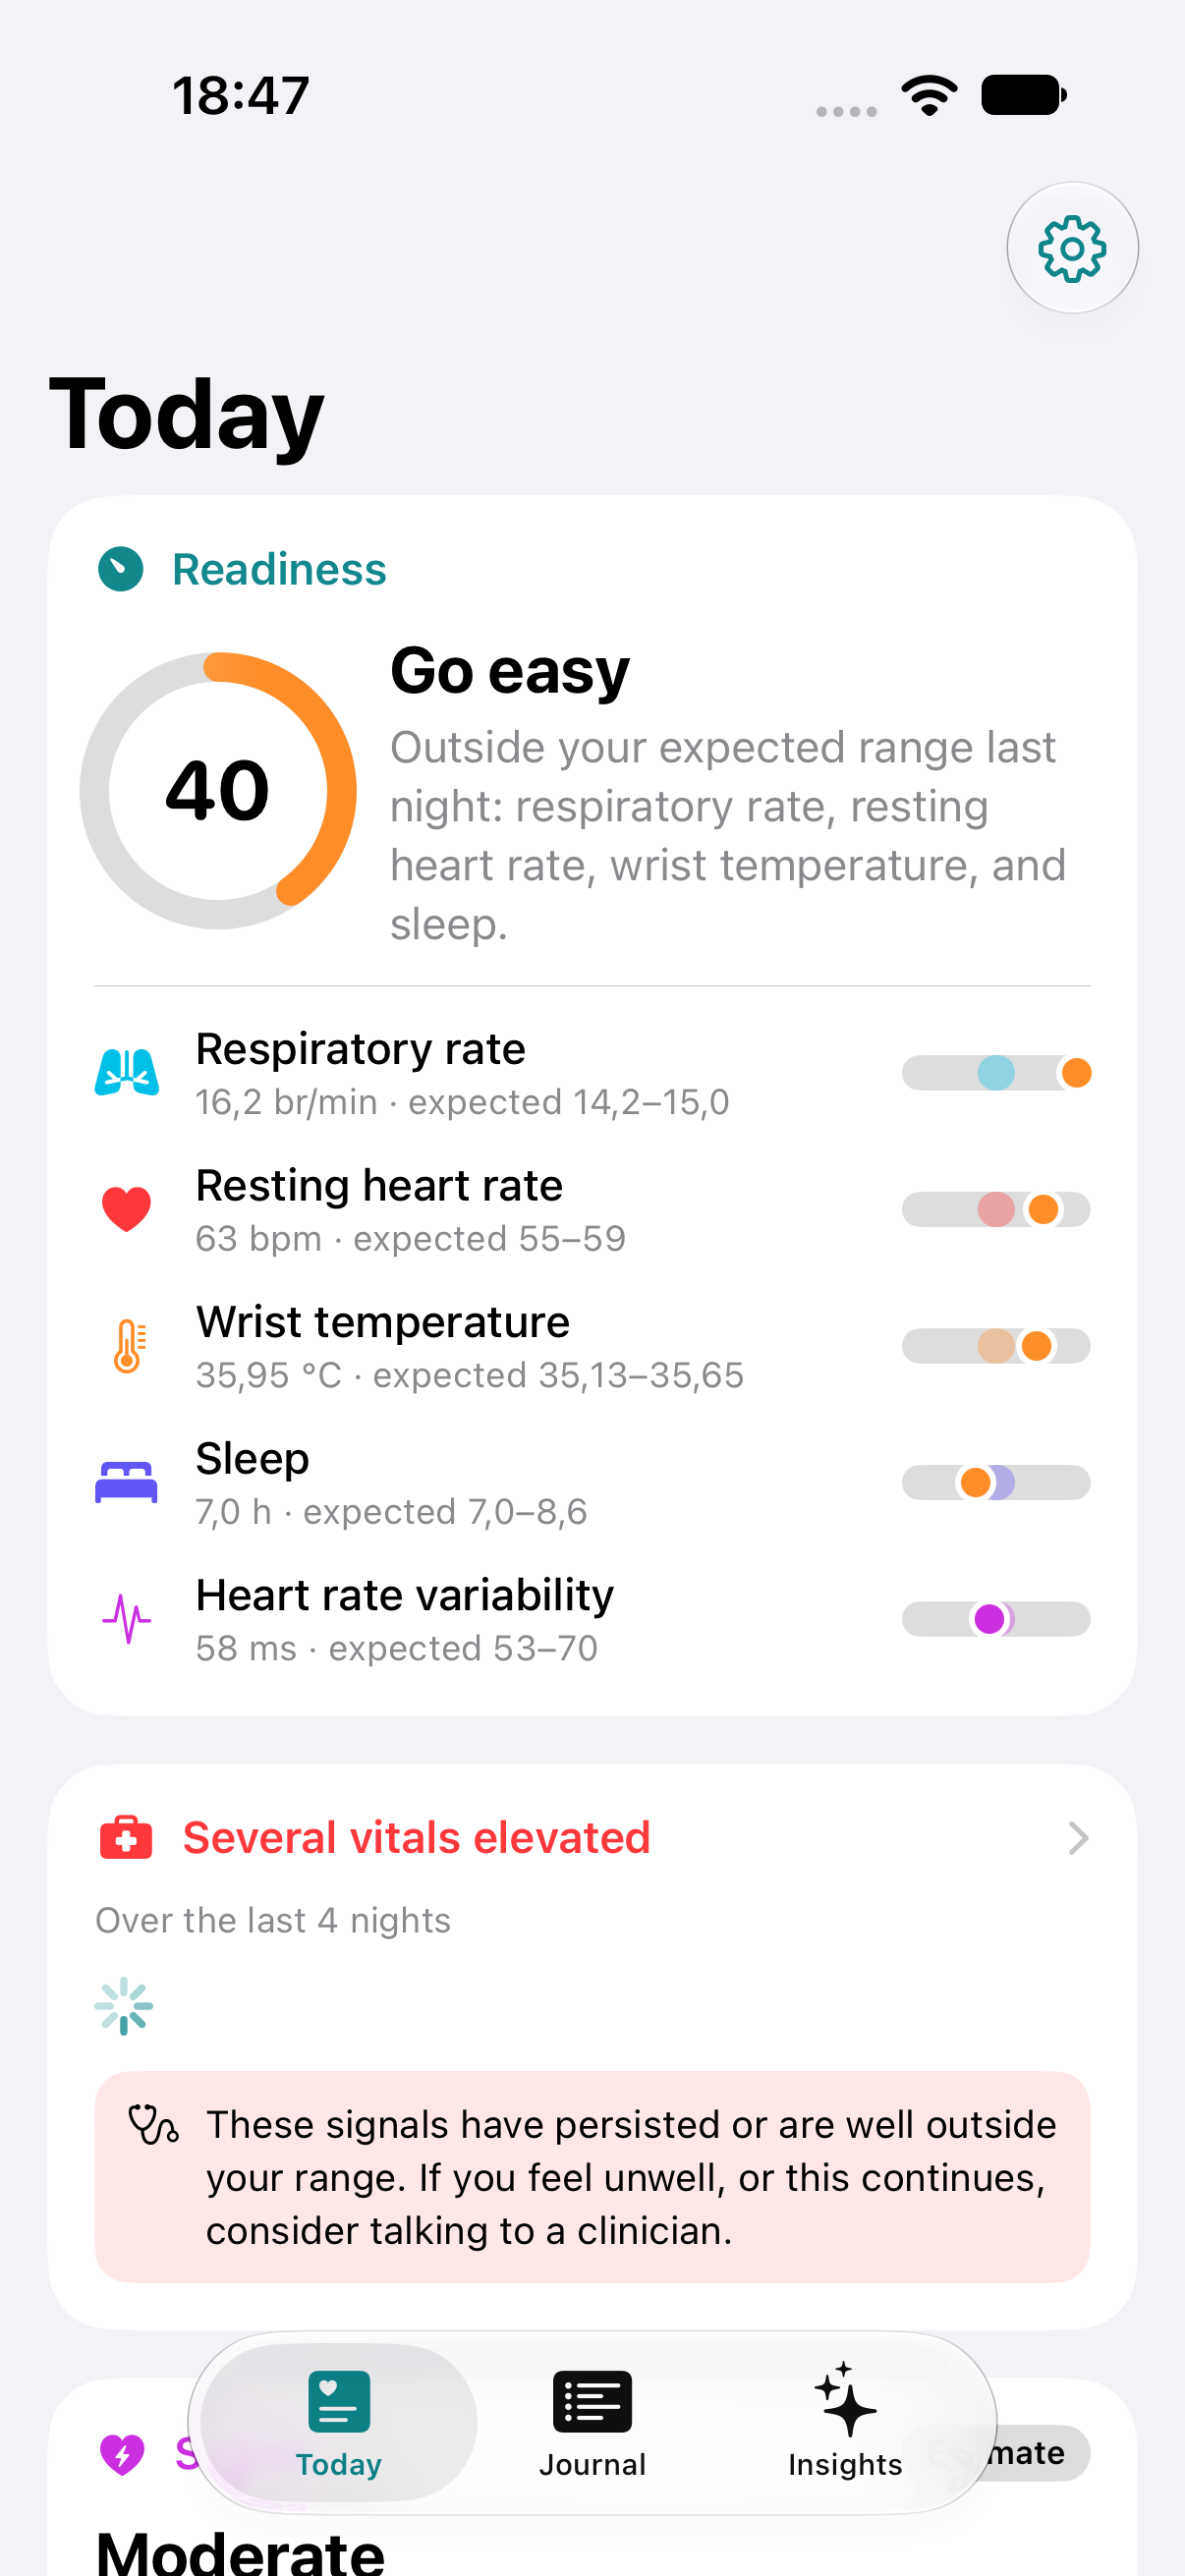
\includegraphics[width=0.19\textwidth]{today.png}\hfill
  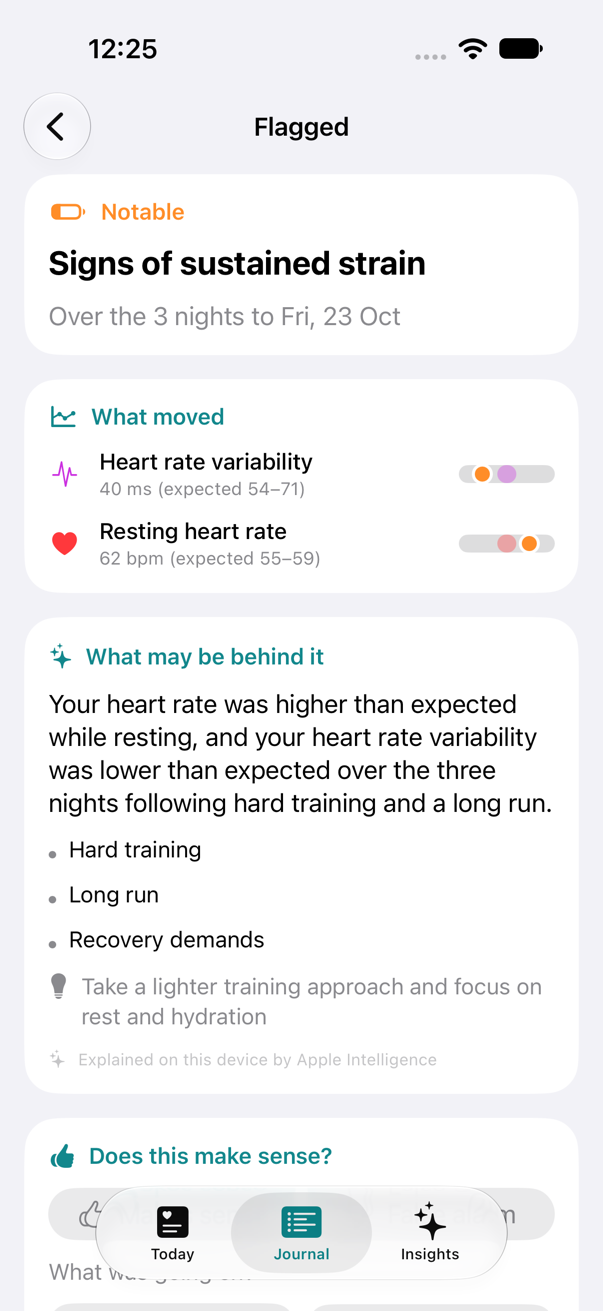
\includegraphics[width=0.19\textwidth]{event.png}\hfill
  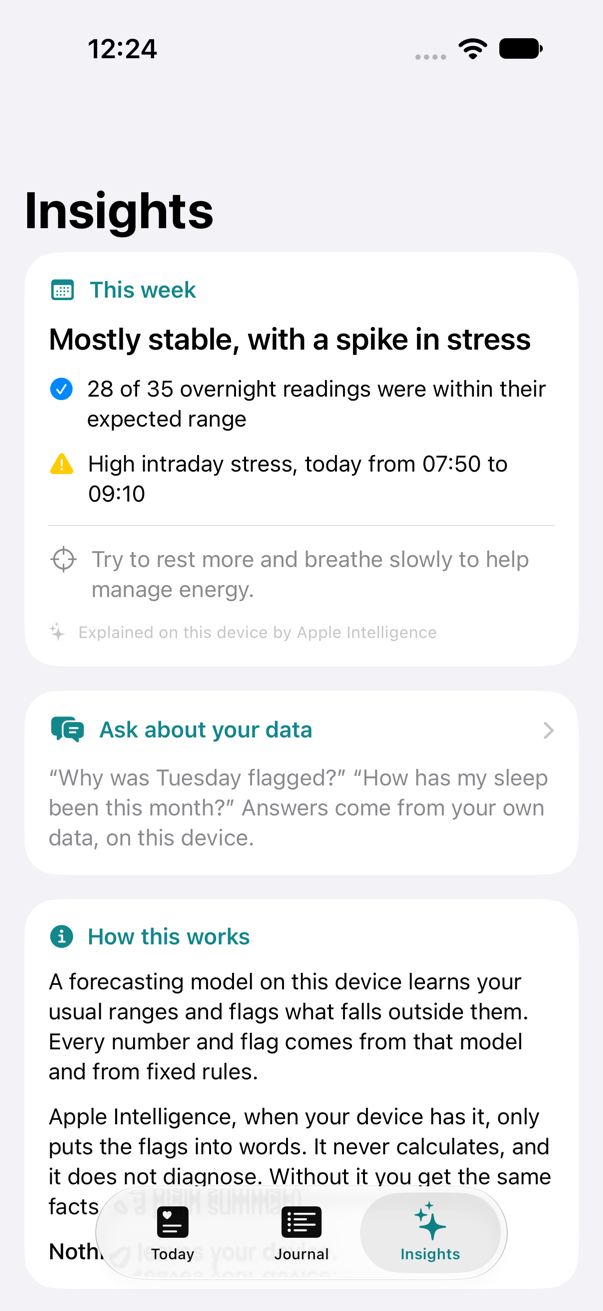
\includegraphics[width=0.19\textwidth]{insights.png}\hfill
  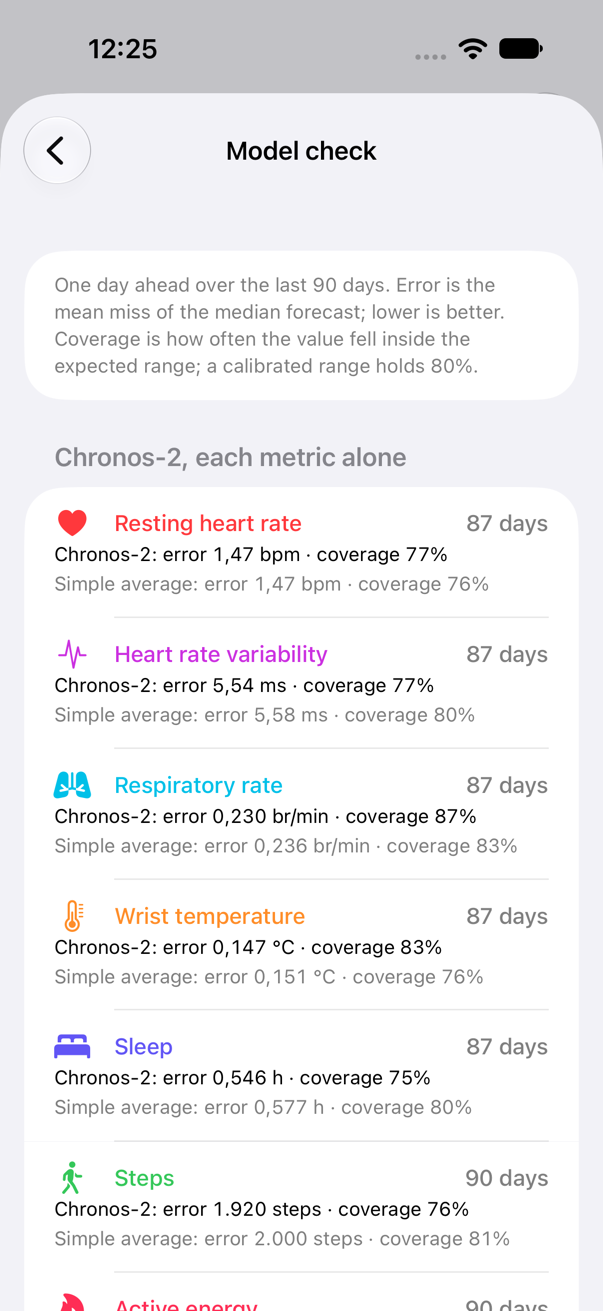
\includegraphics[width=0.19\textwidth]{model-check.png}
  \caption{From left: onboarding (demo data or Apple Health), Today in the sick-week scenario, a flagged event with its explanation, the weekly report, and the model check comparing Chronos-2 with the simple average.}
  \label{fig:screens}
\end{figure}

\subsection{Background updates, notifications and privacy}
A HealthKit observer query and a nightly \texttt{BGProcessingTask} rerun the pipeline when new data arrives. Afterwards the app sends local notifications, each of which the user can switch off: a new event, the morning readiness score, and the weekly report on Mondays. The app contains no network code. Its two files are stored with data protection, and Settings can export the daily values as CSV or erase everything. HealthKit, the forecaster and the language model all run on the device, and no health data leaves it.

% ---------------------------------------------------------------------------
\section{Evaluation}\label{sec:eval}

\subsection{Automated tests}
Table~\ref{tab:tests} summarises the test suite. Package tests use Swift Testing and run on macOS. App-state and UI tests run in the iOS 27.2 simulator on an iPhone 18 Pro profile, and the UI tests also produce the screenshots in this report. Tests that need the language model are enabled only where Apple Intelligence is available, which includes the development Mac and the simulator.

\begin{table}[t]
  \centering\small
  \caption{Automated tests (all passing at the time of writing).}
  \label{tab:tests}
  \begin{tabular}{lrp{9.4cm}}
    \toprule
    Suite & Tests & What they cover \\
    \midrule
    \texttt{ForecastingTests} & 27 & Core ML parity against PyTorch fixtures, frozen ranges, readiness, event rules, stress, backtest \\
    \texttt{InsightsTests} & 27 & Facts and templates, guard rules, question routing, retry messages, advice side per metric, Ask tools; live-model tests for explanations, advice, weekly report, every quick question, triage of greetings, thanks and off-topic questions \\
    \texttt{PersistenceTests} & 4 & Journal and forecast cache across restarts, stored explanations, CSV export, erase \\
    \texttt{HealthDataTests} & 6 & Sleep-night assignment and overlaps, repeatable synthetic scenarios, intraday bins \\
    \texttt{AppTests} & 2 & Replacing a slow Apple Health request with the demo \\
    UI tests & 10 & Every screen on demo data, onboarding, both ways into Apple Health (a round trip through the simulator's Health store), notifications, the learning period, metric advice and Ask \\
    \bottomrule
  \end{tabular}
\end{table}

The live-model tests do not compare against fixed text. They check that the output parses, is non-empty and passes the guard, so they catch a model that stops following the format or starts adding numbers.

\subsection{Forecast accuracy and cost}
On the synthetic person, the model check gives Chronos-2 and the simple average the same error for resting heart rate (1.47 vs 1.47\,bpm mean absolute error) and similar coverage of the q10--q90 band (77\% vs 76\%, nominal 80\%). Joint forecasting with the other metrics as group members gives 1.46\,bpm. This repeats the thesis result~\cite{jankovikj2026chronos}: on a person's own daily series, the foundation model is not more accurate than a moving average. In the app it earns its place in other ways. It gives calibrated ranges from the first few days, it handles missing nights without imputation, it provides the multi-step horizons that frozen ranges need, and one model covers all eight metrics.

A 32-row call takes about 55\,ms natively on an M3 and about 410\,ms in the iOS simulator on the same machine; it has not been timed on an iPhone. The first launch forecasts six months of eight metrics, and Today appears after a few seconds while the rest fills in behind it. Later refreshes forecast one new day per metric.

\subsection{The language model in practice}
The following observations come from development and from the tests against the live model.

\paragraph{The model changes under the app.} The prompts and guard were first tuned on the macOS 26 model. The model shipped with iOS and macOS 27 then skipped the tools for about half of the Ask questions and answered from nothing, fluently: ``nothing was flagged this week'' when something was. Since the model is part of the operating system, an app that relies on it needs regression tests against the live model that are rerun after every OS update. Ours caught this regression.

\paragraph{Routing beats tool choice for a small model.} After a switch from tool calls to routed data in the prompt, answers became specific to the question. We tested on a synthetic week with low HRV, an alcohol log and an illness warning. ``Why is my HRV low?'' was answered with the HRV trend, the short night and the alcohol log. ``How many steps did I take?'' correctly said that no step data was recorded, where the first tool-based version had answered ``318 steps'', which was a workout's calorie count. The guard cannot catch that kind of misattribution, because 318 was in the facts.

\paragraph{Agents need narrow jobs.} Routed data in one prompt had its own failure: every message got an answer about health. ``Hi'' was answered with advice to sleep more, and ``What should I do today?'' with slow breathing, one of the few wellness actions the safety rules allow. The agent split fixes this without giving up routing. Tools came back, but only in the research agent, whose wrong or missing calls are covered by the keyword match. The writer never sees a tool, and a separate triage decides whether to answer at all. Two prompt effects were visible. The writer repeated an example sentence from its instructions word for word (``try going to bed earlier after short sleep''), so the instructions now contain no example sentences. Triage read ``thanks'' as a follow-up when the previous question came first in its prompt, and read it correctly with the message first and the context after it.

\paragraph{Latency.} With the agents run one after another on an M3 Mac, triage takes 0.4--1.2\,s and research 1.2--5.3\,s, one model round trip per tool call. The writer shows its first words after about 1\,s and finishes in about 2\,s. A question about the data is answered in 4--9\,s, and a greeting in about 1\,s. In the simulator the same question took about 40\,s, partly because the model runs one request at a time and the weekly report was still being generated. The Ask screen loads the model when it opens, and the live list of lookups shows progress during the wait.

% ---------------------------------------------------------------------------
\section{Discussion and limitations}

\paragraph{What the design buys.} Separating deciding from wording made every screen work without the language model. It also made the model's output checkable: the guard can only verify numbers and directions because the facts already contain them. The cost is that model output reads somewhat generic. The model tends to repeat the few wellness actions it is allowed, such as rest and slow breathing, and the guard cannot catch vague or loosely rounded sentences. This is why Ask shows its lookups next to every answer.

\paragraph{Limitations.}
\begin{itemize}
  \item \textbf{Synthetic evaluation.} The app has only been evaluated on synthetic data. The thresholds ($2\sigma$, two nights, fourteen nights, the readiness weights) are reasoned defaults, not fitted to real outcomes, and readiness is a heuristic, not a clinical score.
  \item \textbf{No physical device.} Nothing has run on an iPhone or with a real watch's data. HealthKit was tested only with data the app wrote itself, and wrist temperature and workouts cannot be written in the simulator. The nightly background task was never scheduled, because the simulator does not run background tasks; a debug button runs the same update.
  \item \textbf{Ask's safety net and speed.} The research agent's choice of tools is backed up by word lists, so a question that is phrased unusually and also missed by the model gets only the general overview. Three model sessions in a row make answers take seconds, which has not been measured on a phone.
  \item \textbf{The deviation score is unspecific.} As the thesis found, it flags any departure from normal and cannot tell stress from illness from a late night. The event rules and the user's own logs narrow this down, and the app says ``may''.
  \item \textbf{English only}, and not a medical device: the app gives wellness suggestions, not diagnoses.
\end{itemize}

\paragraph{Future work.} The next steps are a field test on real devices that measures on-device latency, battery use and whether flags agree with how users feel; a small study of whether the advice changes behaviour; and fine-tuning or adapting the forecaster on a user's own history, which the thesis left open.

% ---------------------------------------------------------------------------
\section{Conclusion}

Baseline shows that a full personal-health pipeline fits on a phone: HealthKit history, a 28\,MB foundation-model forecaster in Core ML, deterministic rules, and an on-device language model that explains and advises without a server. The forecaster matches its PyTorch reference and is as accurate as a simple average, no more. Its benefit is practical rather than statistical. The language model was most useful when it was given the least to decide. With comparisons, dates and relevance settled by code, it turns an out-of-range reading into a sentence the user can act on, on the screen where they see the value.

\bibliographystyle{plain}
\bibliography{references}

\end{document}
